\chapter{State-of-the-art} % about 20-30 pages
\chaptermark{State-of-the-art of comic books analysis}
\label{chap:sota}
\graphicspath{{./chapters/3-state-of-the-art/figs/}}

% This thesis work has considered symbol spotting problem as an application of subgraph matching. Symbol spotting has experienced a lot of interests among the graphics recognition community. Here the main task starts by querying a given graphic symbol or model object, usually cropped from a bigger document. The main aim is to search the model object in a target document or set of target documents. In this dissertation we will alternatively name the model object to be queried as \emph{model symbol} or \emph{query symbol} or \emph{pattern} and the corresponding graph representing them as \emph{query graph} or \emph{model graph} or \emph{pattern graph}. And the document or the set of documents where the user intends to find the model symbol as \emph{input document} or \emph{target document} and the corresponding graph as \emph{target graph} or \emph{input graph}. Most of the time the user is interested in getting a ranked list of retrieved zones supposed to contain the queried symbol depending on the similarity or dissimilarity measure. This Chapter contains a review of the state-of-the-art of symbol spotting methods. The major existing research can be classified into five broad families as in~\cite{RusinolThesis2009}, which are listed in Table~\ref{table:sota-ss:relworks}. We review those families as follows:

Comics images are mixed content documents that are processed differently depending on the purpose.
The involved techniques can vary a lot between panel, balloon, text and comic character extractions.
We review each of them in the four next subsections.

\section{Panel extraction and layout analysis}
\label{sec:sota:layout_panel}

\begin{itemize}
	% \item Copy/paste from previous publications
	\item Demonstrate that I understand the topic
	\item Conclusion and critics
	% \item Navigating comics: an empirical and theoretical approach to strategies of reading comic page layouts \url{2013_Cohn_navigating_comics.pdf}
	% \item 2013 SIGRAPP poster \url{2013_Tsai_Adaptive Manga Re-Layout On Mobile Device.pdf}
\end{itemize}

Panel extraction and ordering has been mainly studied for panel to panel reading.
The need is increasing since the first generation of mobile devices with small screens in colour or B\&W.
People want to continue reading their favourite comics or manga on the way without caring kilos of books.
Printed comics require tedious work to be manually scanned and split into screen size parts small enough to avoid zooming and scrolling.

Several techniques have been proposed to automatically extract panels as~\cite{In11}, assuming that panels are small enough elements to be comfortably read on mobile devices.
They are based on white line cutting algorithm~\cite{Duda72,li2012automatic,Chan2007Automatic}, recursive X-Y cut~\cite{Han07} or gradient~\cite{Tan07}.
Those methods do not consider empty area~\cite{In11} and border free panel.
These issues have been corrected by connected component approaches~\cite{Arai10} 
%,Rigaud2012LNCS} 
but they are sensible to region that sometimes connect several panels and increase the detection error rate.
Another approach based on morphological mathematics and growing region~\cite{Khoi11} can remove such connecting elements but also create new holes in the panel border.
After the region segmentation step, heuristic filtering is often applied~\cite{Arai11,Khoi11} to classify panel region according to the size ratio with the page which depends on the page format.
More recently, new method have shown interesting results for manga and European comics with different background colours.
They are based on watershed~\cite{ponsard2012ocr}, line segmentation using Canny operator and polygon detection~\cite{Luyuan2014Automatic}, and region of interest detection~\cite{stommel2012segmentation} such as corners~\cite{Tsai2013Adaptive} and line segments.

Page layout analysis have been recently studied to calculate the reading order of the panels.
The page layout influences the reader at choosing pathway~\cite{Cohn_2013}, nevertheless few studies~\cite{Guerin2012Ontologies,Ponsard09,Arai2010Automatic} demonstrated the possibility of calculating such Z-path (left-to-right and down) or right-to-left (e.g. Arabic, Japanese) and down~\cite{Li2013Comic,Tsai2013Adaptive} according to the position of the panels. 

\section{Balloon segmentation and tail detection}
\label{sec:sota:balloon_segmentation}

Balloons or bubbles are the visual unit that conveys dialogue, either spoken or thought.
Balloons have developed into a more-or-less oval shape, with a pointer or tail to indicate to which character they belong.
There are many specialized forms of balloons, either traditional or invented~\cite{Marx2006Writing}.
%Balloons or bubbles are key elements in comics, they link graphical and textual elements and are part of the comics style. 
Few work about balloon detection have been done until now and mainly closed speech balloon have been studied.
Arai~\cite{Arai11} proposed a blob detection method based on connected component detection with four filtering rules for manga.
The rules are based on blob minimum size, white pixel occurrence, inclusion of vertical straight lines detection and width to length ratio (see figure~\ref{fig:Arai_balloon_extraction_process}).
Another connected component approach proposed by Ho~\cite{Ho2012} uses HSV color space to make a first selection of clear blobs and then consider as balloons the blobs with a ratio between the text area and the blob bounding box higher than sixty percent.

From our knowledge, the analysis of open balloons, balloon contour and tails have not been studied before, we propose a first approaches in~\ch{chap:be}.
Those extra information about the balloons are important for a broad understanding of the dialogues and emotions~\cite{millidge2009comic}.

% chapter chap_be (end) ~\ref{sub:be:segmentation}.

%We proposed a first method to extract non closed balloons based on active contours initialized around text areas~\cite{rigaud2013active}, see section~\ref{sub:be:segmentation}.
% This method is able to approximate the contour region, even when it is not printed, based on a domain knowledge which is the mean distance between the balloon contour and the text it contains. 

% A balloon is a spatial container of information that is related to a protagonist using a specific element: the tail.
% The tail is often represented by a discontinuity on contour of the balloon towards the concerned protagonist.
% From our knowledge, there is no work about tail extraction and description in the literature.


%%%%%%%%%%%%%%%%%%%%%%%%%%%%%%%%%%%%%%%%%%%%%%%%%%%
 \begin{figure}[!ht]  %trim=l b r t  width=0.5\textwidth,
   \centering
  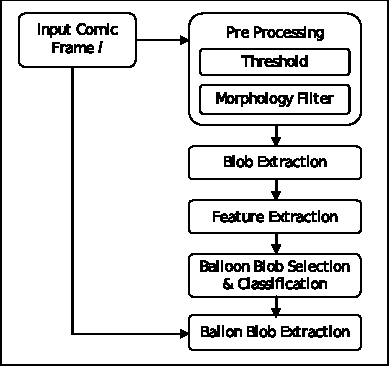
\includegraphics[trim= 0px 0px 0px 0px, clip, width=150px]{figs/Arai_balloon_extraction_process.pdf}
  \caption{Flow diagram of comic balloon detection using comic blob extraction method proposed by Arai~\cite{Arai11}.}
  \label{fig:Arai_balloon_extraction_process}
 \end{figure}
%%%%%%%%%%%%%%%%%%%%%%%%%%%%%%%%%%%%%%%%%%%%%%%%%%%


\section{Text extraction and recognition}
\label{sec:sota:text}

% \begin{itemize}
% 	\item \url{/Text_graphic_separation/2002_Bernhaupt_Using ArtificialNeuralNetwork as image segmentation : application on comics} 
% \end{itemize}


Text extraction and recognition have attracted of lot a attention in document analysis such as newspaper, administrative documents, cheques, maps, floor plans and engineering drawings. 
Nevertheless, the most similar application to comics is car plate recognition~\cite{anagnostopoulos2008license} because the text is in a salient and contrasted area with a complex background around it.
% Nevertheless, plates are typewritten with a fixed length.

%From our knowledge, only text localization has been studied, no text segmentation or text recognition yet. This is probably due to the lack of dataset and ground truth to evaluate the algorithms.
Few work concerns text in comics images, bottom-up approaches use connected component which often relies on the segmentation step~\cite{ponsard2012ocr}.
Su~\cite{Su11} uses Sliding Concentric Windows as text/graphic separation and then apply mathematical morphology and an SVM classifier to classify text from non-text components. 
%Morphological operations are performed with a fixed mask size, the method is orientation and resolution dependent.

% In~\cite{Rigaud2013VISAPP}, we proposed a adaptive binarisation process based on the Minimum Connected Component Thresholding followed by a text/graphic separation based on contrast ratio and text line grouping, see~\ch{chap:te}.
% Previously, we proposed a k-mean classification of the 
Li~\cite{Li2013Unsupervised} proposed an unsupervised speech text localization for comics that trains a Bayesian classifier on aligned connected component and then detect the rest of the text using the classifier for text/non text separation.
 

% Rigaud~\cite{Rigaud12} %~\cite{Rigaud12}
% make use of ``the median value of the border page pixels'' to binarize the image, extract CC and then classify them into ``noise'', ``text'' or ``frame'' (based on CC heights). This method assumes that the page always contains text and that the text background colour is similar to the paper background. 

Top-down approaches starting from balloons (white blobs) detection followed by mathematical morphology operations have been proposed by Arai~\cite{Arai11} and Yamada~\cite{Yam04} and Sundaresan~\cite{Sundaresan2012Text}.



\section{Comic character detection}
\label{sec:sota:comic_character}

\begin{itemize}
	\item Garfield character detector based on color histogram \url{/PhD/Biblio_LINK/Object_detection2013_Landry_Color Based Comic Strip Character Recognition.pdf}
	\item \url{2011_Matsui_Interactive manga retargeting - siggraph11.pdf}
	\item \url{object/2012_Takayama_FACE DETECTION AND FACE RECOGNITION
OF CARTOON CHARACTERS USING FEATURE EXTRACTION}
	\item \url{object/2007_MASTER_Cheung_Face detection and face recognition of human-like characters in comics}
	\item Stoke images \url{Object_detection/2010_THESIS_Ta_phuong_inexact_graph_matching_application_to_stroke_images_comics.pdf}
\end{itemize}

\section{Holistic understanding} % (fold)
\label{sec:sota:holistic_understanding}

% section holistic_understanding (end)

\section{Existing applications}
\label{sec:sota:applications}

\begin{itemize}
	\item \url{http://vomic.shueisha.co.jp/}
	\item Comic Chat is a working program, allowing groups of people to communicate over the Internet see \url{2006_Kurlander_Comic_Chat.pdf}
	\item \url{2010_Tobita_Comic Engine: Interactive System for Creating and Browsing Comic books with Attention Cuing.pdf}
	\item Online interactive creation of comics \url{2009_Lopes_Calligraphic Shortcuts for Comics Creation.pdf}
	\item \url{2010_Tobita_Comic Engine: Interactive System for Creating and Browsing Comic books with Attention Cuing}
	\item Software for scripting comics, to define the interactions, time, zoom and region for a kind of video export \url{2012_Raulet_A Sketch-based Interface to Script Comics Reading.pdf}
	\item Movie to comics: ... the first three factors determine balloon size, and the last factor determines balloon shape ... Emotion can be further exhibited by shape of balloon [1] \url{/PhD/Biblio_LINK/Speech_balloon_analysis/2013_Chu_Optimized Speech Balloon Placement for Automatic_comics_generation.pdf}
\end{itemize}

\section{Conclusion}
\label{sec:sota:conclusion}

% To conclude the literature review, some of the challenges of symbol spotting can be highlighted from the above state-of-the-art reviews. First, symbol spotting is concerned with various graphical documents viz. electronic documents, architectural floorplans etc., which in reality suffer from \emph{noise} that may come from various sources such as low-level image processing, intervention of text, etc. So efficiently handling structural noise is crucial for symbol spotting in documents. Second, an example application of symbol spotting is to find any symbolic object from a large amount of documents. Hence, the method should be efficient enough to handle a \emph{large database}. Third, symbol spotting is usually invoked by querying a cropped symbol from some document, which acts as a query to the system. So it implies infinite possibilities of the query symbols, and indirectly \emph{restricts the possibility of training} in the system. Finally, since symbol spotting is related to real-time applications, the method should have a \emph{low computational complexity}. We chose these five important aspects (segmentation, robustness in noise, training free, computational expenses, robustness with a large database) of symbol spotting to specify the advantages and disadvantages of the key research, which is listed in Table~\ref{table:sota-ss:relworkscomp}.

% In the next chapter, we are going to propose the first symbol spotting algorithm. The method is based on the factorization of graph into serialized subgraphs (graph paths) and then organizing those graph paths into hash table. The hash based technique helps to reduce search space considerably and perform the subgraph matching (symbol spotting) faster.